\documentclass[a4paper,12pt]{article}

%\begin{figure}[htp]
%    \centering
%    \includegraphics[width=0.75\textwidth]{}
%\end{figure}

%%%%%%%%%%%%%%%%%%%%
%%%%  PREAMBLE  %%%%
%%%%%%%%%%%%%%%%%%%%
\usepackage{float}
\usepackage[T1]{fontenc}
\usepackage[utf8]{inputenc}

\usepackage[english,italian]{babel}
\usepackage{graphicx}     % Per includere immagini
\usepackage{subcaption}   % Per utilizzare subfigure
\usepackage{hyperref}
\usepackage{indentfirst}

\hypersetup{hidelinks}

\usepackage[margin=2.5cm]{geometry}
\usepackage{minipage-marginpar}
\usepackage{fancyhdr}
\usepackage[bottom]{footmisc}
\usepackage{lastpage}

\usepackage{enumitem}
\usepackage{tabularx}

\usepackage{graphicx}

\setlength{\parindent}{0em}
\setlength{\parskip}{1em}

\fancyhead[L]{\leftmark}
\fancyhead[R]{\shortstack[r]{Versione documento: 0.01 \\ Gruppo: G24}}

\fancyfoot[C]{}
\fancyfoot[R]{\thepage/\pageref{LastPage}}

\renewcommand{\headrulewidth}{2pt}
\renewcommand{\headruleskip}{3pt}
\setlength{\headheight}{30pt}

\renewcommand{\footrulewidth}{2pt}

\setlist[itemize]{itemsep=0.25em,topsep=0pt}
\setlist[enumerate]{itemsep=0.25em,topsep=0pt,align=left}

%%%%%%%%%%%%%%%%%%%%
%%%%  DOCUMENT  %%%%
%%%%%%%%%%%%%%%%%%%%

\title{}
\author{Gruppo G24}

\begin{document}

\pagestyle{empty}

\begin{center}

    \vspace{2 cm}

    \begin{tabular*}{\textwidth}{ c @{\extracolsep{\fill}} c }
        
\includegraphics[width=0.3\textwidth]{marchio_unitrento.pdf} & \shortstack{\Large{Dipartimento di Ingegneria} \\ \Large{e Scienza dell'Informazione}}
    \end{tabular*}

    \vspace{5 cm} 
  
    \Huge \textbf{Ingegneria del software\\}
  
    \vspace{1.5 cm} 
    \Large\textsc{Documento di specifica dei requisiti tramite UML\\} 
    \vspace{3 cm} 
    \Huge\textsc{Mountain Wonders\\}
    \Large{Gruppo G24}
  
    \vspace{2 cm} 
  
    \Large{Anno accademico 2023/2024}
\end{center}

\newpage
\tableofcontents

\pagestyle{fancy}
\newpage
\section{Scopo del documento}

Il presente documento riporta la specifica dei requisiti di sistema del progetto MountainWonders. Lo scopo di questo documento è quello di mostrare le specifiche dei requisiti funzionali e non funzionali tramite l'utilizzo di diagrammi UML (Unified Modeling Language), diagrammi degli use-case, tabelle, context diagram e component diagram.\\
All'interno del documento precedentemente consegnato, sono stati specificati i requisiti funzionali e non funzionali in linguaggio naturale, mentre ora verranno espressi utilizzando un linguaggio più formale e strutturato.
    
\newpage

\section{Requisiti funzionali}

Vengono elencati di seguito i requisiti funzionali(RF) dell'applicazione, tramite l'utilizzo degli Use Case Diagram.

\subsection*{RF5 Account anonimo}

\subsubsection*{RF1 Registrazione}
\begin{figure}[H]
   \centering
    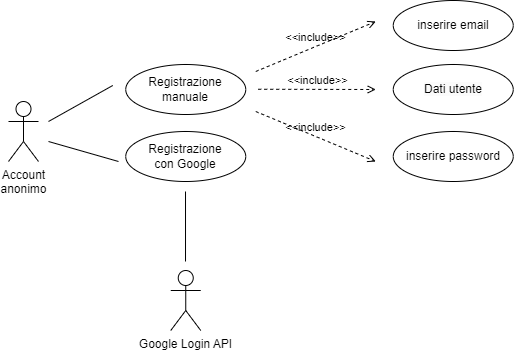
\includegraphics[width=0.8\textwidth]{img/registrazione_anonimo.png}
    \caption{USE-CASE Registrazione}
\end{figure}

Questo USE-CASE rappresenta la registrazione dell'utente Anonimo.
E' possibile effettuare la registrazione manuale, inserendo i dati richiesti, oppure utilizzare un account google esistente.

\begin{figure}[H]
   \centering
    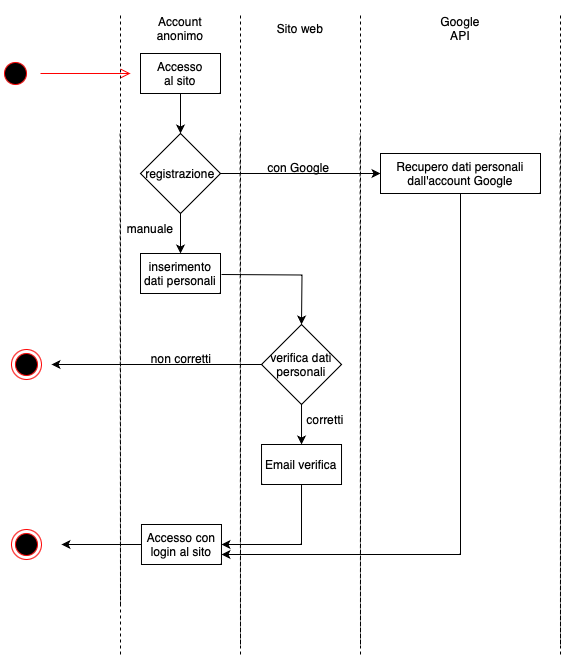
\includegraphics[width=0.90\textwidth]{img/diagramma_registrazione.png}
    \caption{Diagramma attività registrazione}
\end{figure}

Questo diagramma delle attività rappresenta il processo di registrazione dell'utente Anonimo. 
Arrivato alla pagina di registrazione, l'utente potrà scegliere tra le due modalità presenti.

Se viene scelta la registrazione tramite google, l'utente viene reindirizzato ad un'altra pagina e, una volta scelto l'account, ritornerà automaticamente sul sito.

Se invece si sceglie la registrazione manuele, sarà necessario inserire indirizzo email, password e alcuni dati (nome, cognome); La password deve rispettare dei requisiti per essere considerata sicura (RNF1).
Una volta inseriti i dati, l'utente riceverà, all'indirizzo email specificato, un link per verficare il suo account. 


\subsubsection*{RF2 Login}
\begin{figure}[H]
   \centering
   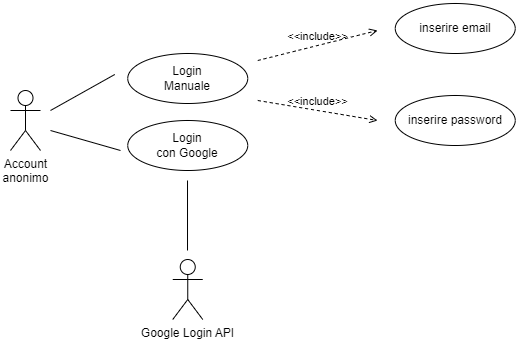
\includegraphics[width=0.8\textwidth]{img/login_anonimo.png}
    \caption{USE-CASE Login}
\end{figure}

Questo USE-CASE rappresenta il login dell'utente Anonimo.
E' possibile effettuare il login manuale, inserendo indirizzo email e password, oppure utilizzare il proprio account google.

\begin{figure}[H]
   \centering
    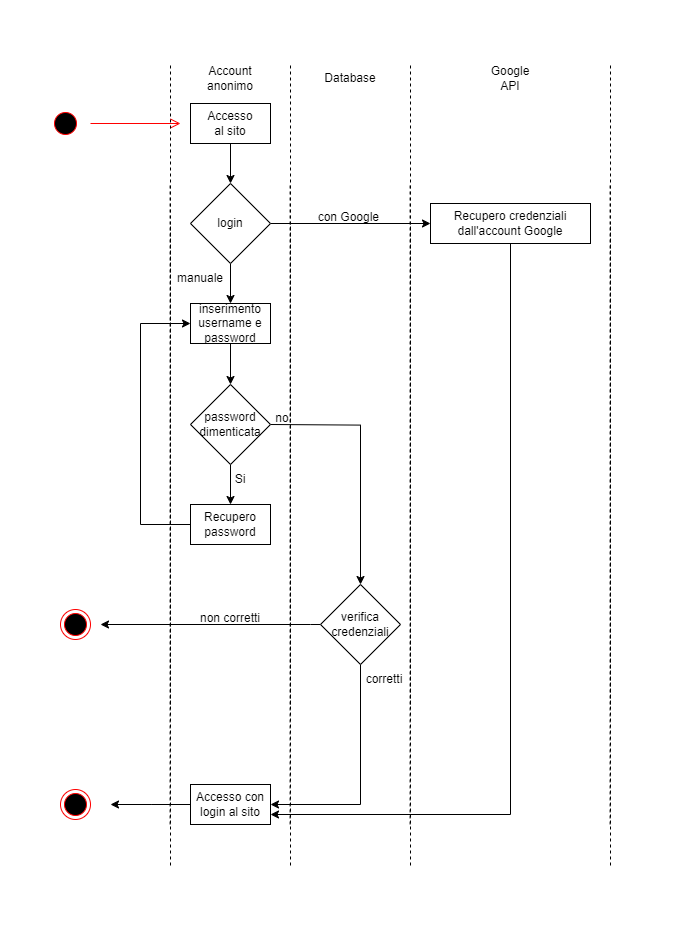
\includegraphics[width=1\textwidth]{img/diagramma_login.png}
    \caption{ Diagramma attività login}
\end{figure}

Questo diagramma delle attività rappresenta il processo di login dell'utente Anonimo. 
Arrivato alla pagina di login, l'utente potrà scegliere tra le due modalità presenti.

Se viene scelta la registrazione tramite google, l'utente viene reindirizzato ad un'altra pagina e, una volta scelto l'account, ritornerà automaticamente sul sito.

Se invece si sceglie il login manuale, sarà necessario inserire indirizzo email e password.
L'utente ha la possibilità, in questa pagina, di recuperare la password; In questo caso riceverà un'email con un link per cambiare password.
Se indirizzo email e password sono corretti, l'utente accede al sito.


\subsubsection*{RF8 Ricerca}
\begin{figure}[H]
   \centering
   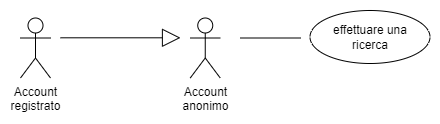
\includegraphics[width=0.7\textwidth]{img/ricerca.png}
    \caption{USE-CASE Ricerca}
\end{figure}

Questo USE-CASE rappresenta la ricerca di un rifugio o di una montagna.
Il sito utilizzerà le perole chiave fornite dall'utente per trovare una corrispondenza all'interno del database.
E' possibile effettuare la ricerca sia dall'account anonimo, che dall'account registrato.

\subsubsection*{RF7.1 Visualizza recensioni, RF9 Visualizzare montagne-rifugi}
\begin{figure}[H]
   \centering
   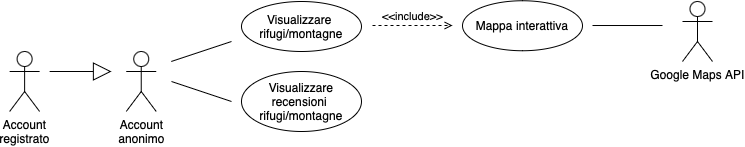
\includegraphics[width=1.0\textwidth]{img/visualizzare_montagne.png}
    \caption{USE-CASE Visualizza Montagne-Rifugi-Recensioni}
\end{figure}


\subsubsection*{RF11 Supporto}
\begin{figure}[H]
   \centering
   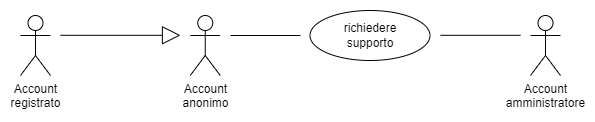
\includegraphics[width=1\textwidth]{img/richiesta_supporto.png}
    \caption{USE-CASE Richiesta supporto}
\end{figure}

\subsubsection*{RF12 Cambio lingua}
\begin{figure}[H]
   \centering
   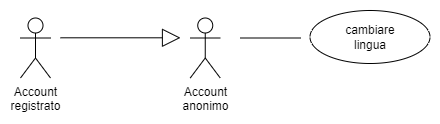
\includegraphics[width=0.8\textwidth]{img/cambio_lingua.png}
    \caption{USE-CASE Cambio lingua}
\end{figure}

Questo USE-CASE rappresenta la possibilità di cambiare lingua.
Sarà presente un menù, nella parte superiore di ogni pagina, che permetterà di cambiare lingua a preferenza dell'utente. 
Questo menu elenca tutte le lingue supportate, quali italiano, inglese, tedesco.

\subsubsection*{RF13 Meteo della Montagna}
\begin{figure}[H]
   \centering
   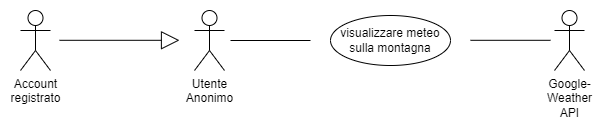
\includegraphics[width=1\textwidth]{img/meteo.png}
    \caption{USE-CASE Meteo montagna}
\end{figure}

\subsection*{RF3 Account Amministratore}
\subsubsection*{RF2 Login amministratore}
\begin{figure}[H]
   \centering
   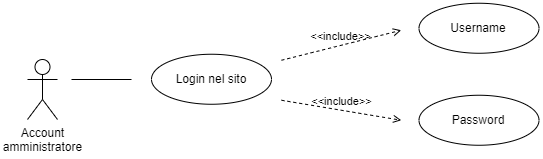
\includegraphics[width=0.8\textwidth]{img/login_amministratore.png}
    \caption{USE-CASE Login}
\end{figure}

Questo USE-CASE rappresenta il login dell'utente Amministatore.
In questo caso, a differenza dell'utente Anonimo, e' possibile solamente effettuare il login manuale, inserendo username e password dell'account Amministratore preesistente. 

\subsubsection*{RF3.1 Eliminare utenti registrati}
\begin{figure}[H]
   \centering
   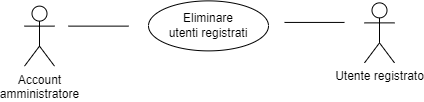
\includegraphics[width=0.6\textwidth]{img/eliminazione_utenti.png}
    \caption{USE-CASE Eliminazione utenti}
\end{figure}

\subsubsection*{RF3.2 Eliminare recensioni}
\begin{figure}[H]
   \centering
   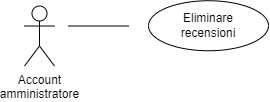
\includegraphics[width=0.4\textwidth]{img/eliminazione_recensioni.png}
    \caption{USE-CASE Eliminazione recensioni}
\end{figure}

Questo USE-CASE rappresenta l'eliminazione delle recensioni da parte dall'account Amministratore.
Alcune informazioni potrebbero essere già presenti (ridondanza della pagina) oppure la recensione potrebbe contenere dei contenuti inappropriati. 
In questi casi, nella sezione delle recensioni di una montagna o di un rifugio, sarà presente un pulsante per eliminare una recensione.

\subsubsection*{RF3.3 Modificare/Eliminare montagna o rifugio}
\begin{figure}[H]
   \centering
   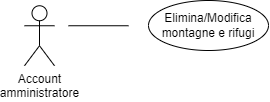
\includegraphics[width=0.4\textwidth]{img/m_e_montagna_rifugio.png}
    \caption{USE-CASE Modifica/Eliminazione montagne e/o rifugi}
\end{figure}

Questo USE-CASE rappresenta l'eliminazione delle montagne o rifugi da parte dall'account Amministratore.
Come nel caso delle recensioni, alcune informazioni potrebbero essere ridondate oppure contenere contenuti inappropriati, l'amministratore avrà la possibilità di eliminare una montagna dal sistema.
Oltre all'eliminazione delle informazioni della montagna, vengono eliminate anche le recensioni legate ad essa. 

\subsubsection*{RF3.4 Rispondere alle richieste di supporto}

\begin{figure}[H]
   \centering
   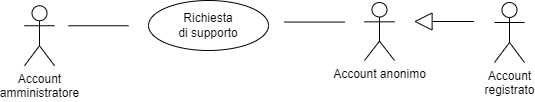
\includegraphics[width=0.8\textwidth]{img/richiesta_supporto_amministratore.png}
    \caption{USE-CASE Risposta alla richiesta di supporto}
\end{figure}

\subsubsection*{RF3.5 Inserire montagna}
\begin{figure}[H]
   \centering
   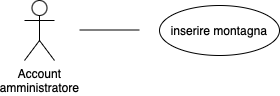
\includegraphics[width=0.4\textwidth]{img/inserire_montagna.png}
    \caption{USE-CASE Inserire montagna}
\end{figure}
Questo USE-CASE rappresenta l'inserimento di nuove montagne non ancora registrate sul sito da parte dall'account Amministratore.
Consentirà di inserire tutte le informazioni relative ad esse.


\subsection*{RF4 Account registrato}

Di seguito vengono descritte le funzioni dell'account registrato.

\subsubsection*{RF7 Recensioni}
\begin{figure}[H]
   \centering
   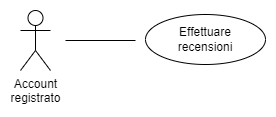
\includegraphics[width=0.4\textwidth]{img/recensioni_registrato.png}
    \caption{USE-CASE Recensioni}
\end{figure}

Questo USE-CASE rappresenta l'inserimento di una recensione da parte dell'account registrato.
Nella pagina di visualizzazione di un rifugio, sarà presente una sezione per inserire la propria recensione.
 
\subsection*{RF6 Profilo utente}
\begin{figure}[H]
   \centering   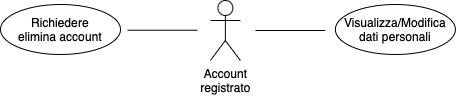
\includegraphics[width=0.5\textwidth]{img/profilo_utente.png}
    \caption{USE-CASE Profilo utente}
\end{figure}

Questo USE-CASE rappresenta la visualizzazione e la modifica del profilo utente da parte dell'account registrato.
Nella pagina del profilo personale, sarà possibile visualizzare e modificare le informazioni del proprio profilo (nome, cognome, indirizzo email, password, foto profilo).
Sarà inoltre possibile richiedere l'eliminazione dell'account dal sistema. 


\subsection*{RF10 Aggiungere rifugio}
\begin{figure}[H]
   \centering   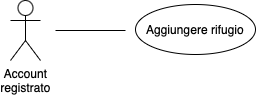
\includegraphics[width=0.4\textwidth]{img/aggiungere_rifugio.png}
    \caption{USE-CASE Aggiungere rifugio}
\end{figure}
Sarà possibile a tutti gli utenti registrati l'inserimento di un nuovo rifugio.

\subsection*{Use case totale}
\begin{figure}[H]
   \centering
    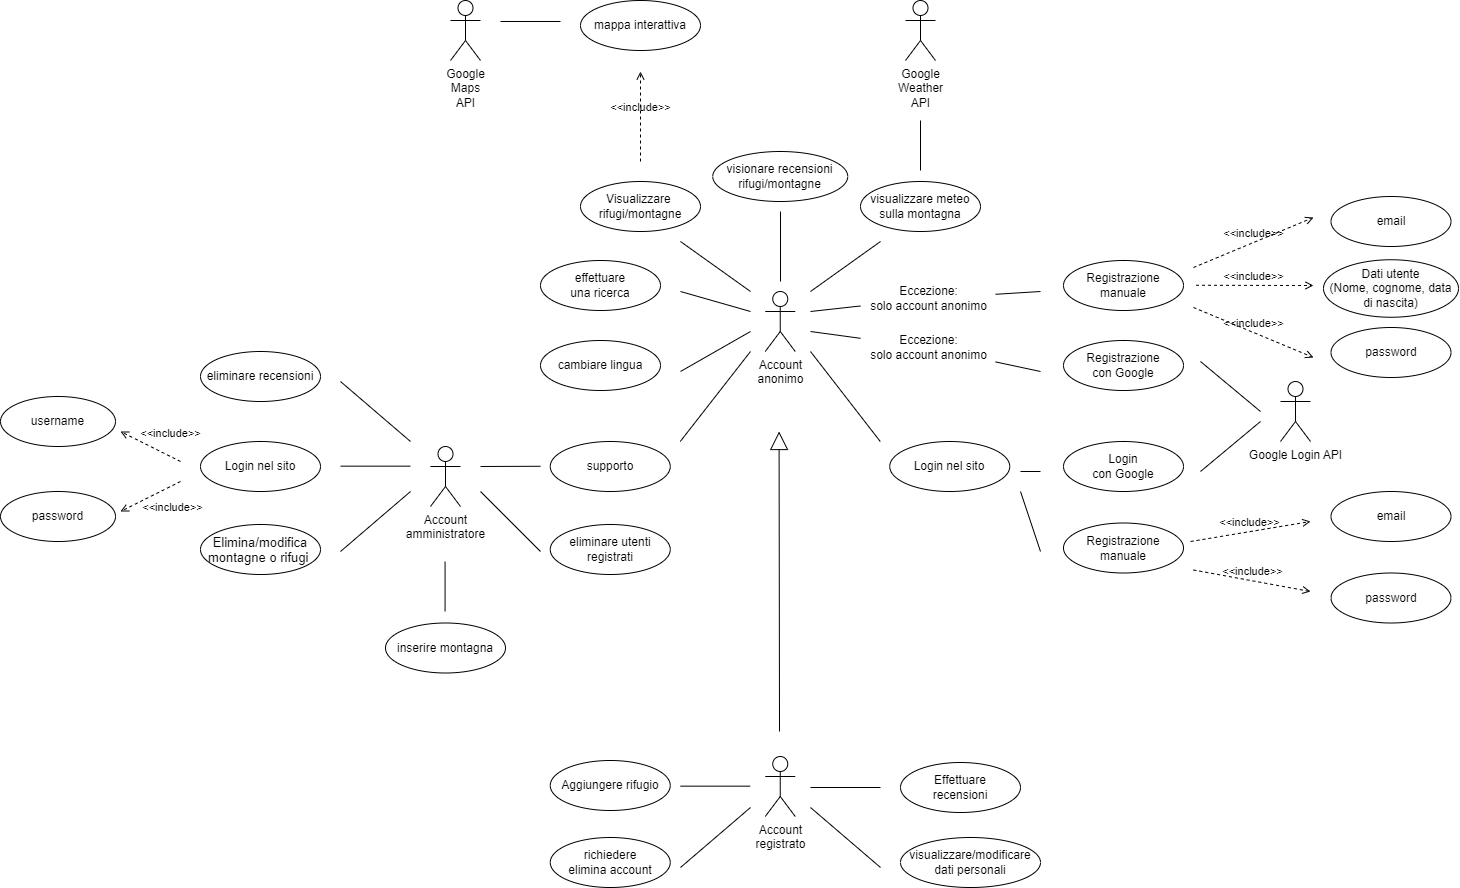
\includegraphics[width=1.29\textwidth, angle = 90]{img/use_case_completo.png}
    
\end{figure}
Eccezioni:
\begin{itemize}
    \item La registrazione manuale la può fare solo un utente anonimo
    \item La registrazione con Google la può fare solo un utente anonimo
\end{itemize}{}



{\newpage}
\section{Requisiti non funzionali}

Vengono di seguito elencati e descritti i requisiti non funzionali del progetto. Ciascun requisito diversamente dai requisiti funzionali è legato alle performance.\\
Per ogni requisito funzionale, viene fatta una descrizione a cui viene accompagnata una misura, per poter verificare se il requisito funzionale è stato soddisfatto o meno.

\subsection*{RNF1 Sicurezza}

\begin{table}[H]
    \centering
    \begin{tabular}{|p{0.2\textwidth}|p{0.38\textwidth}|p{0.38\textwidth}|}
    

        \hline 
         Proprietà & Descrizione & Misura\\
         \hline      
         
         Password sicure&  Gli utenti associano un username al proprio account e una password sicura che permette la protezione dei propri dati personali& Una password sicura deve avere una lunghezza minima di 8 caratteri, lettere sia maiuscole che minuscole, inoltre devono essere presenti almeno un carattere speciale (\&, £, \$, \#, ...) e almeno un numero.\\ \hline
        Utilizzo TLS/SSL & Tutti i dati sensibili degli utenti, come informazioni personali e password, saranno crittografati sia in transito, sia quando il dato non viene utilizzato
        per l’accesso & Il link della pagina deve contenere https all'inizio di esso, ossia un protocollo per la comunicazione sicura attraverso Internet. La trasmissione verrà effettuata sulla porta 443 (standard per l'https). \\  \hline
        Email verificata & L’indirizzo email inserito dall’utente deve essere verificato &
        Quando l'utente effettua la registrazione, oppure elimina il proprio account, un'email di verifica viene inviata per confermare l'identità.
        \\ \hline
    \end{tabular}

    \caption{Sicurezza}
\end{table}

\subsection*{RNF2 Performance}

\begin{table}[H]
    \centering
    \begin{tabular}{|>{\centering}p{0.2\textwidth}|p{0.38\textwidth}|p{0.38\textwidth}|}
        \hline  
         Proprietà & Descrizione & Misura\\
         \hline      
         Performance  
         &Il sito deve essere in grado di gestire il numero richiesto di utenti senza alcun degrado delle prestazioni. Deve essere inoltre veloce e rendere gradibile la navigazione.
         &  Le performance vengono stabilite da il tempo di risposta dopo un’operazione dell’utente, per garantire alte performance il tempo massimo di rispsota sarà di 2 secondi.\\ \hline
    \end{tabular}
    \caption{Performance}
    
\end{table}


\subsection*{RNF3 Compatibilità}
\begin{table}[H]
    \centering
    \begin{tabular}{|p{0.2\textwidth}|p{0.38\textwidth}|p{0.38\textwidth}|}
        
         \hline  
         Proprietà & Descrizione & Misura\\
         \hline
         Compatibilità
         & Gli utenti devono poter accedere al sito web tramite l'utilizzo di qualisiasi dispositivo,  tra computer, tablet e smartphone, utilizzando uno dei browser supportati.
         & Il sito web deve essere supportato nel 95\% dei dispositivi.\\ \hline
    \end{tabular}
    
    \caption{Compatibilità}
\end{table}


\subsection*{RNF4 Affidabilità e disponibilità}
\begin{table}[H]
    \centering
    \begin{tabular}{|p{0.2\textwidth}|p{0.38\textwidth}|p{0.38\textwidth}|}
         \hline  
         Proprietà & Descrizione & Misura\\
         \hline 
            Affidabilità
         &  i dati inseriti dagli utenti verranno salvati all’interno di un database. Su questi verranno effettuati backup, per poter eventualmente recuperare i dati in caso di guasti del sistema o di attacchi informatici.
         & I backup verranno eseguiti ogni 7 giorni.\\ \hline
         Disponibilità & La disponibilità del sito è la capacità di essere accessibile agli utenti in qualsiasi momento, Per garantire un'ottima disponibilità del sito sarà necessario un ottimo servizio di hosting con strutture ridondanti. & Il sito dovrà essere disponibile almeno 23 ore al giorno, 7 giorni a settimana. \\ \hline
    \end{tabular}
    \caption{Affidabilità e disponibilità}
\end{table}


\subsection*{RNF5 Usabilità}
\begin{table}[H]
    \centering
    \begin{tabular}{|p{0.2\textwidth}|p{0.38\textwidth}|p{0.38\textwidth}|}
        \hline  
         Proprietà & Descrizione & Misura\\
         \hline      
         Usabilità
         & Gli utenti devono essere in grado di saper utilizzare il sito web in maniera completa senza bisogno di dover utilizzare alcun manuale, in breve tempo.
         &Un utente deve essere in grado di utilizzare completamente il sito dopo 15 minuti.\\ \hline
    \end{tabular}
    \caption{Usabilità}
\end{table}


\subsection*{RNF6 Norme recensioni}
\begin{table}[H]
    \centering
    \begin{tabular}{|p{0.2\textwidth}|p{0.38\textwidth}|p{0.38\textwidth}|}
        \hline  
         Proprietà & Descrizione & Misura\\
         \hline      
         Norme recensioni
         & Le recensioni devono essere conformi a norme contro discriminazioni o blasfemie.
         &Le recensioni che conterranno discriminazioni o blasfemie verranno eliminate dall'account amministratore.\\ \hline
    \end{tabular}
    \caption{Norme recensioni}
\end{table}

\subsection*{RNF7 Gestione delle immagini}
\begin{table}[H]
    \centering
    \begin{tabular}{|p{0.2\textwidth}|p{0.38\textwidth}|p{0.38\textwidth}|}
        \hline  
         Proprietà & Descrizione & Misura\\
         \hline      
         Gestione immagini
         & Le immagini devono essere gestite in modo da non provocare un rallentamento del sito web.
         &La massima dimensione delle immagini caricate dagli utenti è di 3MB.\\ \hline
    \end{tabular}
    \caption{Gestione immagini}
\end{table}


\subsection*{RNF8 Privacy}
\begin{table}[H]
    \centering
    \begin{tabular}{|p{0.2\textwidth}|p{0.38\textwidth}|p{0.38\textwidth}|}
        \hline  
         Proprietà & Descrizione & Misura\\
         \hline      
         GDPR
         & Il sito raccoglierà e tratterà dati
        personali degli utenti, dopo aver fornito avvisi chiari sulla privacy e acquisito i consensi necessari.
         &Conforme\\ \hline
         Copyright
         & Sarà rispettato il copyright per tutti i contenuti utilizzati sul sito.
         &Sarà avitato l’uso non autorizzato di testi, immagini e altri materiali protetti.\\ \hline
         COPPA
         & Il sito effettuerà un controllo dell’età dell’utente che si registra.
         &L'utente che si registra deve avere minimo 13 anni.\\ \hline
    \end{tabular}
    \caption{Privacy}
\end{table}


\subsection*{RNF9 Aggiornamenti} 
\begin{table}[H]
    \centering
    \begin{tabular}{|p{0.2\textwidth}|p{0.38\textwidth}|p{0.38\textwidth}|}
        \hline  
         Proprietà & Descrizione & Misura\\
         \hline      
         Aggiornamenti
         & Il sito web sarà sviluppato con un'infrastruttura scalabile, per garantire l'aggiunta di nuove funzionalità e il miglioramento complessivo dell'esperienza utente.
         & Una volta al mese verrà effettuato un controllo sull'adeguatezza dell'architettura, e in caso verranno effettuati opportuni aggiornamenti.\\ \hline
    \end{tabular}
    \caption{Aggiornamenti}
\end{table}
 


\newpage

\section{Diagramma di contesto}
Il diagramma di contesto fornisce una visione chiara delle interazioni tra il sistema, gli utenti registrati e l'amministratore. 

\subsection{Descrizione}

\begin{enumerate}
    \item Attori: Ci sono tre attori principali identificati:
    \begin{itemize}
        \item Utente Anonimo (RF5)
        \item Amministratore (RF3)
        \item MountainsWonders (il sistema centrale)
        \item Mail Service
        \item Google login API 
        \item Database
    \end{itemize}
    
    \item Interazioni Utente Anonimo - MountainsWonders:  
    \begin{itemize}
        \item L'Utente Anonimo può registrarsi direttamente attraverso il sito o tramite Google.(RF1) 
        \item Può effettuare l'accesso sia usando le credenziali del sito sia tramite Google.(RF2)
        \item L'Utente Anonimo può richiedere il reset della password.
        \item Può effettuare ricerche e visualizzare montagne o rifugi basandosi sui risultati di tali ricerche. (RF8)
        \item Può richiedere supporto e ricevere una risposta. (RF11)
    \end{itemize}
    
    \item Interazioni Amministratore - MountainsWonders:
    \begin{itemize}
        \item L'Amministratore può effettuare l'accesso. (RF2)
        \item Può ricevere messaggi di richiesta di supporto e fornire risposte. (RF3.4)
    \end{itemize}
    
    \item Interazioni MountainsWonders - Database:
    \begin{itemize}
        \item Tramite le interazioni con il database il sito si occupa della registrazione, l'autenticazione, le ricerche e altre funzioni correlate. (RF1, RF2, RF8)
    \end{itemize}
    
    \item Interazioni MountainsWonders - Servizi Esterni:
    \begin{itemize}
        \item MountainsWonders comunica con un servizio di posta elettronica per inviare email.
        \item Utilizza Google Login API per gestire l'autenticazione tramite Google. (RF1, RF2)
    \end{itemize}
    
\end{enumerate}

\begin{figure}[H]
   \centering   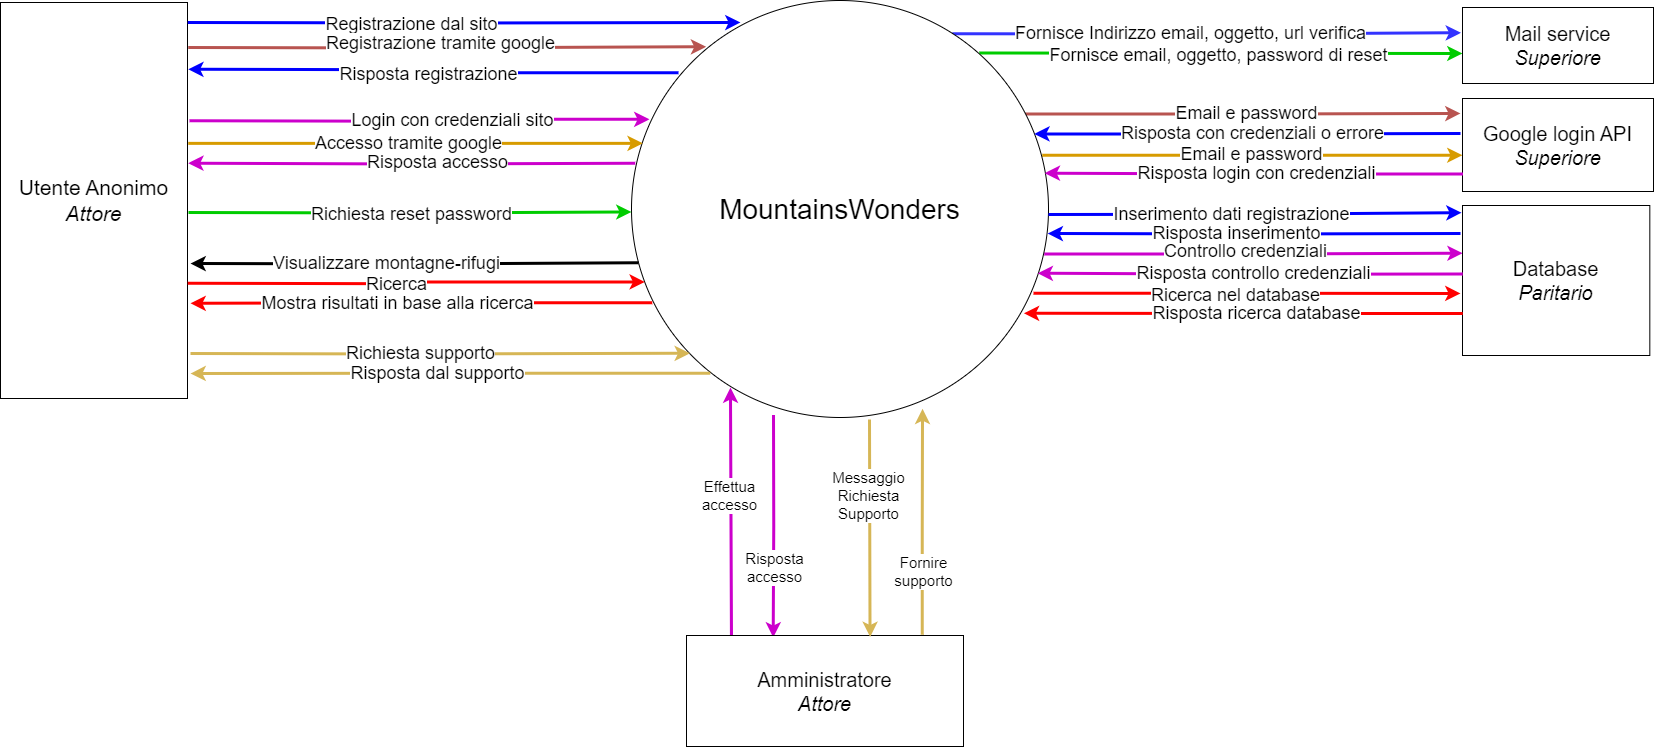
\includegraphics[width=1.0\textwidth]{img/contesto_anonimo.png}
    \caption{Diagramma di contesto Utente Anonimo}
\end{figure}



\subsection{Descrizione}
Analizziamo il contenuto del secondo diagramma di contesto:




\begin{enumerate}
    \item Attori: Ci sono tre attori principali identificati:
    \begin{itemize}
        \item Utente Registrato (RF4)
        \item Amministratore (RF3)
        \item MountainsWonders (il sistema centrale)
    \end{itemize}


    
    \item Interazioni Utente Registrato - MountainsWonders:
    \begin{itemize}
        \item L'Utente Registrato può richiedere la visualizzazione dei propri dati personali e ricevere una risposta. (RF6)
        \item Ha la possibilità di modificare i propri dati personali e ricevere un feedback sulla modifica. (RF6) 
        \item Può inserire rifugi e ricevere una conferma sull'inserimento.
        \item Ha la possibilità di inserire o eliminare recensioni e ricevere un feedback su tali azioni. (RF7)
        \item Può visualizzare le recensioni effettuate. (RF6) 
        \item  Ha la possibilità di richiedere l'eliminazione del proprio account e ricevere una risposta in merito. (RF6)
    \end{itemize}

    
    \item Interazioni Amministratore - MountainsWonders:
    \begin{itemize}
        \item Può eliminare utenti (RF3.1)
        \item Elimina recensioni effettuate dagli utenti (RF3.2)
        \item Può ricevere messaggi di richiesta di supporto e fornire risposte. (RF3.4)
    \end{itemize}
    
    \item Interazioni MountainsWonders - Servizi Esterni:
    \begin{itemize}
        \item  MountainsWonders interagisce con il databse per propagre le operazioni fatte dall'utente e dall'amministratore.
        
    \end{itemize}
\end{enumerate}




\begin{figure}[H]
   \centering   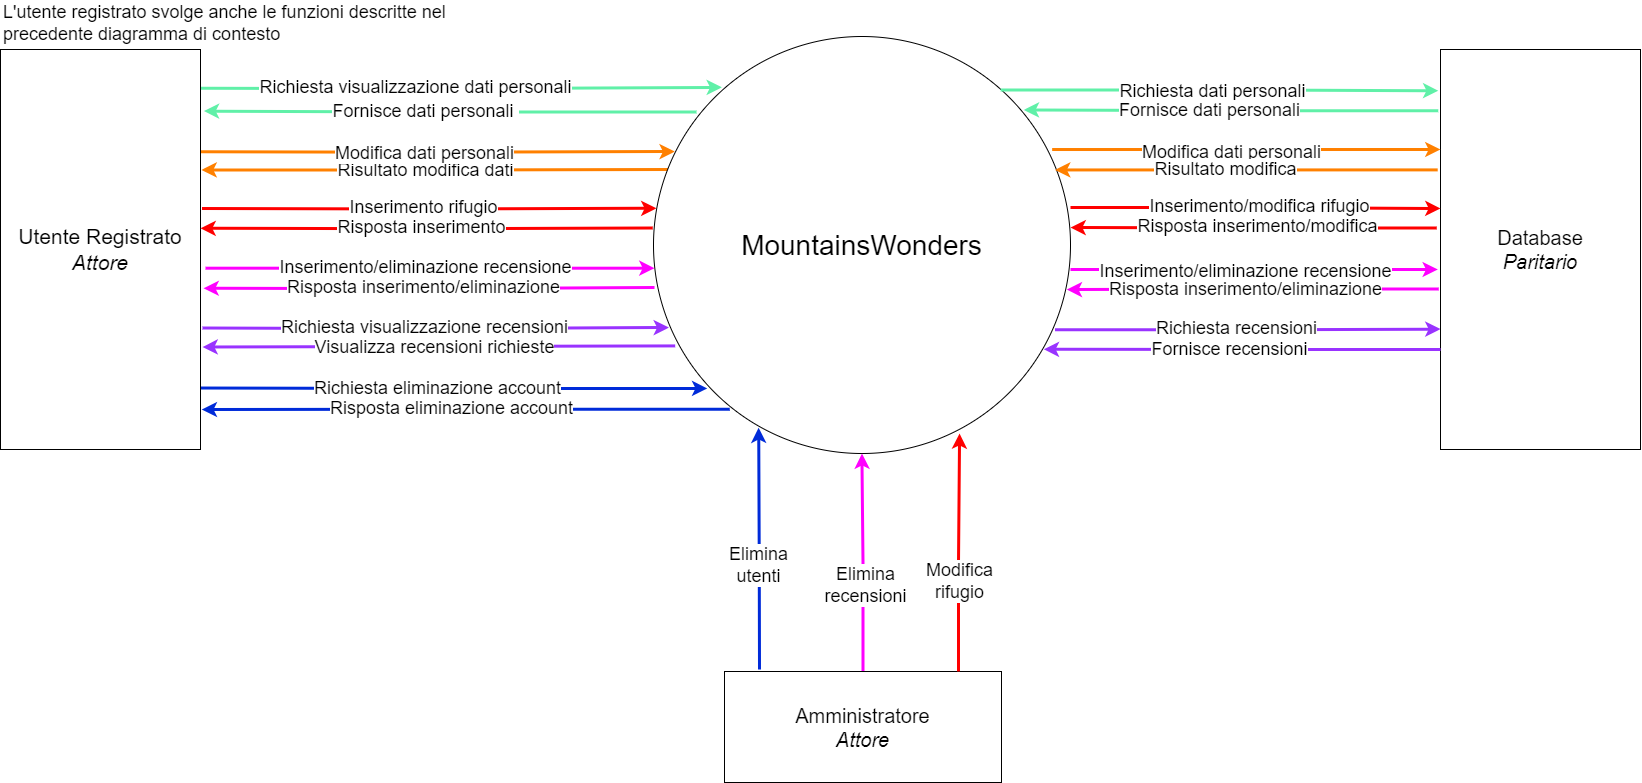
\includegraphics[width=1.0\textwidth]{img/contesto_registrato.png}
    \caption{Diagramma di contesto Utente Registrato}
\end{figure}
\newpage
\section{Diagramma delle componenti}
Andiamo ad analizzare le diverse componenti che costituiscono il nostro sistema, considerando il contesto in cui esse si integreranno. Questa analisi comprenderà una descrizione dettagliata di ciascuna componente, inclusi i suoi punti di ingresso e uscita, e si concluderà con la creazione di un diagramma delle componenti.


\subsection{Analisi delle componenti}

\subsubsection{Pagina supporto}
\underline{Descrizione}: questa componente permette ad un utente di richiedere supporto all'amministratore.

\underline{Interfacce richieste:}
\begin{itemize}
\item Richiesta supporto: questa interfaccia permette di raccogliere i dati presenti nella richiesta di supporto effettuata dall'utente per poi essere utilizzati dall'amministratore (RF11).
\end{itemize}

\underline{Interfacce fornite:}
\begin{itemize}
\item Risposta supporto: questa interfaccia permette di inviare all'utente la risposta dell'amministratore alla richiesta di supporto(RF11).
\end{itemize}



\subsubsection{Homepage}
\underline{Descrizione}: questa componente si occupa della prima interazione da parte di un utente con il sito web.
  
\underline{Interfacce fornite:} 
\begin{itemize}
    \item Accesso: questa interfaccia permette ad un utente di effettuare l'accesso al sito, tramite l'utilizzo di una diversa componente (RF2).
    \item Richiesta di supporto: questa interfaccia permette di ridirezionare l'utente ad una nuova pagina per la richiesta di supporto all'amministratore (RF11).
    \item Visualizzazione montagne: questa interfaccia permette di ridirezionare l'utente ad una nuova pagina per la visualizzazione delle montagne (RF9).
    \item Visualizza rifugi: questa interfaccia permette di ridirezionare l'utente ad una nuova pagina per la visualizzazione dei rifugi(RF9).
\end{itemize}



\subsubsection{Pagina montagne}
\underline{Descrizione}: questa componente si occupa di fornire all'utente l'elenco delle montagne presenti all'interno del database esterno (RF9).

\underline{Interfacce richieste:}
\begin{itemize}
\item Visualizzazione montagne: questa interfaccia permette di recuperare la scelta fatta dall'utente per indirizzarlo alla pagina corretta, ossia la pagina che fornisce l'elenco delle montagne.
\item Dati montagne database: questa interfaccia permette di recuperare l'elenco delle montagne e dei relativi dettagli dal database esterno (RF9).
\end{itemize}

\underline{Interfacce fornite:}
\begin{itemize}
\item Elenco montagne: questa interfaccia fornisce l'elenco delle montagne disponibili con i relativi dettagli (RF9). 
\end{itemize}



\subsubsection{Pagina inserimento montagna}
\underline{Descrizione}: questa componente permette all'amministratore di inserire una nuova montagna (RF3.5).

\underline{Interfacce richieste:}
\begin{itemize}
\item Descrizione montagna: questa interfaccia rappresenta una breve descrizione della montagna, inserita dall'amministratore.
\item Immagine: questa interfaccia rappresenta un'immagine della montagna, inserita dall'amministratore (RF3.5).
\item Aggiunta montagna: questa interfaccia permette di reindirizzare l'amministratore alla pagina per l'aggiunta di una nuova montagna all'interno del database, operazione eseguita tramite l'utilizzo di un'altra componente.
\end{itemize}

\underline{Interfacce fornite:}
\begin{itemize}
\item Montagna: questa interfaccia fornisce la montagna inserita dall'amministratore in modo che possa essere poi visualizzata all'interno della componentente "Pagina montagne" (RF9).
\end{itemize}



\subsubsection{Pagina rifugi}
\underline{Descrizione}: questa componente si occupa di recuperare e fornire all'utente l'elenco dei rifugi presenti all'interno del database esterno (RF9).

\underline{Interfacce richieste:}
\begin{itemize}
\item Visualizzazione rifugi: questa interfaccia permette di recuperare la scelta fatta dall'utente per indirizzarlo alla pagina corretta, ossia la pagina che fornisce l'elenco dei rifugi(RF9).
\item Dati rifugi database: questa interfaccia permette di recuperare l'elenco di rifugi e dei relativi dettagli dal database esterno.
\item Eliminazione rifugio: questa interfaccia all'amministratore di eliminare un rifugio  (RF3.3).
\end{itemize}

\underline{Interfacce fornite:}
\begin{itemize}
\item Elenco rifugi: questa interfaccia permette di fornire l'elenco dei rifugi disponibili con i relativi dettagli (RF9).
\item Aggiunta recensione: questa interfaccia permette di reindirizzare l'utente alla pagina per l'inserimento di una nuova recensione, operazione che verrà gestita da un'altra componente.
\item Aggiunta rifugio: questa interfaccia permette di reindirizzare l'utente alla pagina per l'inserimento di un nuovo rifugio, che verrà gestito da un'altra componente (RF10).
\end{itemize}



\subsubsection{Pagina inserimento rifugio}
\underline{Descrizione}: questa componente permette a un utente di inserire un nuovo rifugio(RF10).

\underline{Interfacce richieste:}
\begin{itemize}
\item Descrizione rifugio: questa interfaccia rappresenta una breve descrizione del rifugio, inserita dall'utente.
\item Immagine: questa interfaccia rappresenta un'immagine del rifugio, inserita dall'utente.
\item Aggiunta rifugio: questa interfaccia permette di reindirizzare l'utente alla pagina per l'inserimento di un nuovo rifugio, che verrà gestito da un'altra componente (RF10).
\end{itemize}

\underline{Interfacce fornite:}
\begin{itemize}
\item Rifugio: questa interfaccia fornisce il rifugio inserito dall'utente in modo che possa essere poi visualizzato all'interno della componentente "Pagina Rifugi".
\end{itemize}



\subsubsection{Accesso account}
\underline{Descrizione}: questa componente si occupa della registrazione di nuovi utenti (RF1) e del login degli utenti (RF2). I dati ricevuti verranno trasmessi alle altre componenti.

\underline{Interfacce richieste:} 
\begin{itemize}
    \item Accesso: questa interfaccia si occupa di reindirizzare l'utente nella sezione per effettuare l'accesso ad un account dopo aver premuto un bottone nell'homepage (RF2).
    \item Email, password e dati personali: queste componenti sono necessarie per l'accesso di un utente o per la sua registrazione (RF1).
\end{itemize}

\underline{Interfacce fornite:} 
\begin{itemize}
    \item Login utente: questa interfaccia propaga i dati del login fornendoli alle altre componenti che si occuperanno della verifica.
    
    \item Registrazione utente: questa interfaccia fornisce i dati della registrazione.Verranno verificati da altre componenti.
\end{itemize} 



\subsubsection{Verifica credenziali}
\underline{Descrizione}: questa componente si occupa della verifica delle credenziali. Verrà effettuato un controllo che confronterà i dati inseriti con quelli presenti nel database. Questa componente si occupa anche della propagazione dei dati personali nelle altre componenti.

\underline{Interfacce richieste:} 
\begin{itemize}
    \item Login utente: questa interfaccia richiede i dati di login degli utenti che verranno poi verificati dall'interfaccia.
    \item Registrazione utente: questa interfaccia si occupa di verificare email, sicurezza della password e i dati personali e controlla la presenza nel database dell'email.   
\end{itemize}

\underline{Interfacce fornite:} 
\begin{itemize}
    \item Credenziali utente: questa interfaccia fornisce le credenziali utente alle altre componenti che li richiedono.
\end{itemize} 



\subsubsection{Pagina utente}
\underline{Descrizione}: questa componente si occupa di fornire tutti i dettagli di un determinato utente (RF6).

\underline{Interfacce richieste:}
\begin{itemize}
\item Credenziali utente: questa interfaccia recupera le credenziali di un utente dal database esterno per permettere di visualizzare i relativi dati personali (RF6).
\item Dati personali: questa interfaccia permette di recuperare i dati personali relativi all'utente dal database esterno per poterli visualizzare (RF6).
\item Nuovi dati personali: questa interfaccia contiene i nuovi dati personali inseriti dall'utente che andranno poi a sostituire quelli originali presenti all'interno del database esterno, qualora fosse necessario apportare delle modifiche (RF6).
\end{itemize}

\underline{Interfacce fornite:}
\begin{itemize}
\item Dati utente: questa interfaccia fornisce all'utente i suoi dati, qualora volesse verificarne la correttezza e/o modificarli.
\item Visualizza recensioni: questa componente permette di reindirizzare l'utente ad una nuova pagina per visualizzare le recensioni da lui effettuate (RF7.1).
\end{itemize}



\subsubsection{Pagina recensioni}
\underline{Descrizione}: questa componente si occupa di fornire all'utente l'elenco delle recensioni da lui fatte (RF7.1).

\underline{Interfacce richieste:}
\begin{itemize}
\item Recupero recensione database: questa interfaccia recupera i dati delle nuove recensioni inserite in modo poi che un'altra interfaccia possa usarli.
\item Visualizza recensioni: questa interfaccia recupera la scelta dell'utente, ossia quella di essere reindirizzato alla pagina delle recensioni (RF7.1). 
\item Elimina recensione: questa interfaccia recupera la scelta dell'amministrazione per eliminare una recensione (RF3.1).
\end{itemize}

\underline{Interfacce fornite:}
\begin{itemize}
\item Recensioni: questa interfaccia fornisce l'elenco delle recensioni eseguite da un utente, in modo che questi dati possano essere utilizzati da un'altra componente.
\end{itemize}



\subsubsection{Pagina inserimento recensione}
\underline{Descrizione}: questa componente permette ad un utente di aggiungere una nuova recensione riguardo un rifugio.

\underline{Interfacce richieste:}
\begin{itemize}
\item Aggiunta recensione: questa interfaccia permette reindirizzare l'utente verso la pagina per l'aggiunta di una recensione .
\item Descrizione recensione: questa interfaccia permette di recuperare dal database esterno tutte le descrizioni  di ogni singola recensione eseguita dall'utente.
\item Valutazione: questa interfaccia permette di recuperare dal database esterno tutte le valutazioni di ogni singola recensione eseguita dall'utente.
\item Dati utente: questa componente dovrà recuperare i dati dell'utente che sta inserendo la nuova recensione.
\end{itemize}

\underline{Interfacce fornite:}
\begin{itemize}
\item Recensione: questa interfaccia permette di inviare i dati della nuova recensione ad un'altra componente in modo da poterli usare per visualizzare l'elenco delle recensioni.
\end{itemize}



\subsubsection{Pagina amministratore}
\underline{Descrizione}: questa componente fornisce tutti i dettagli dell'utente amministratore (RF3).

\underline{Interfacce richieste:}
\begin{itemize}
\item Credenziali utente: questa interfaccia permette di reindirizzare l'utente verso la pagina con i relativi permessi per l'amministratore.
\item Descrizione recensione: questa interfaccia permette di recuperare dal database esterno tutte le descrizioni  di ogni singola recensione eseguita dall'utente.
\end{itemize}

\underline{Interfacce fornite:}
\begin{itemize}
\item Risposta richiesta: questa interfaccia permette di inviare la risposta ad una richiesta di supporto alle altri componenti da parte dell'amministratore.
\item Eliminazione recensione: questa componente permette l'eliminazione di una recensione che non rispetta i determianti criteri (RNF6).
\item Aggiunta montagna: questa componente consente l'aggiunta di nuove montagne (RF3.3)
\item Eliminazione rifugio: questa interfaccia permette di eliminare un rifugio nel caso non rispetti i criteri o esista un duplicato (RF3.3)
\end{itemize}


\subsection{Diagramma componenti:}
\begin{figure}[H]
   \centering
   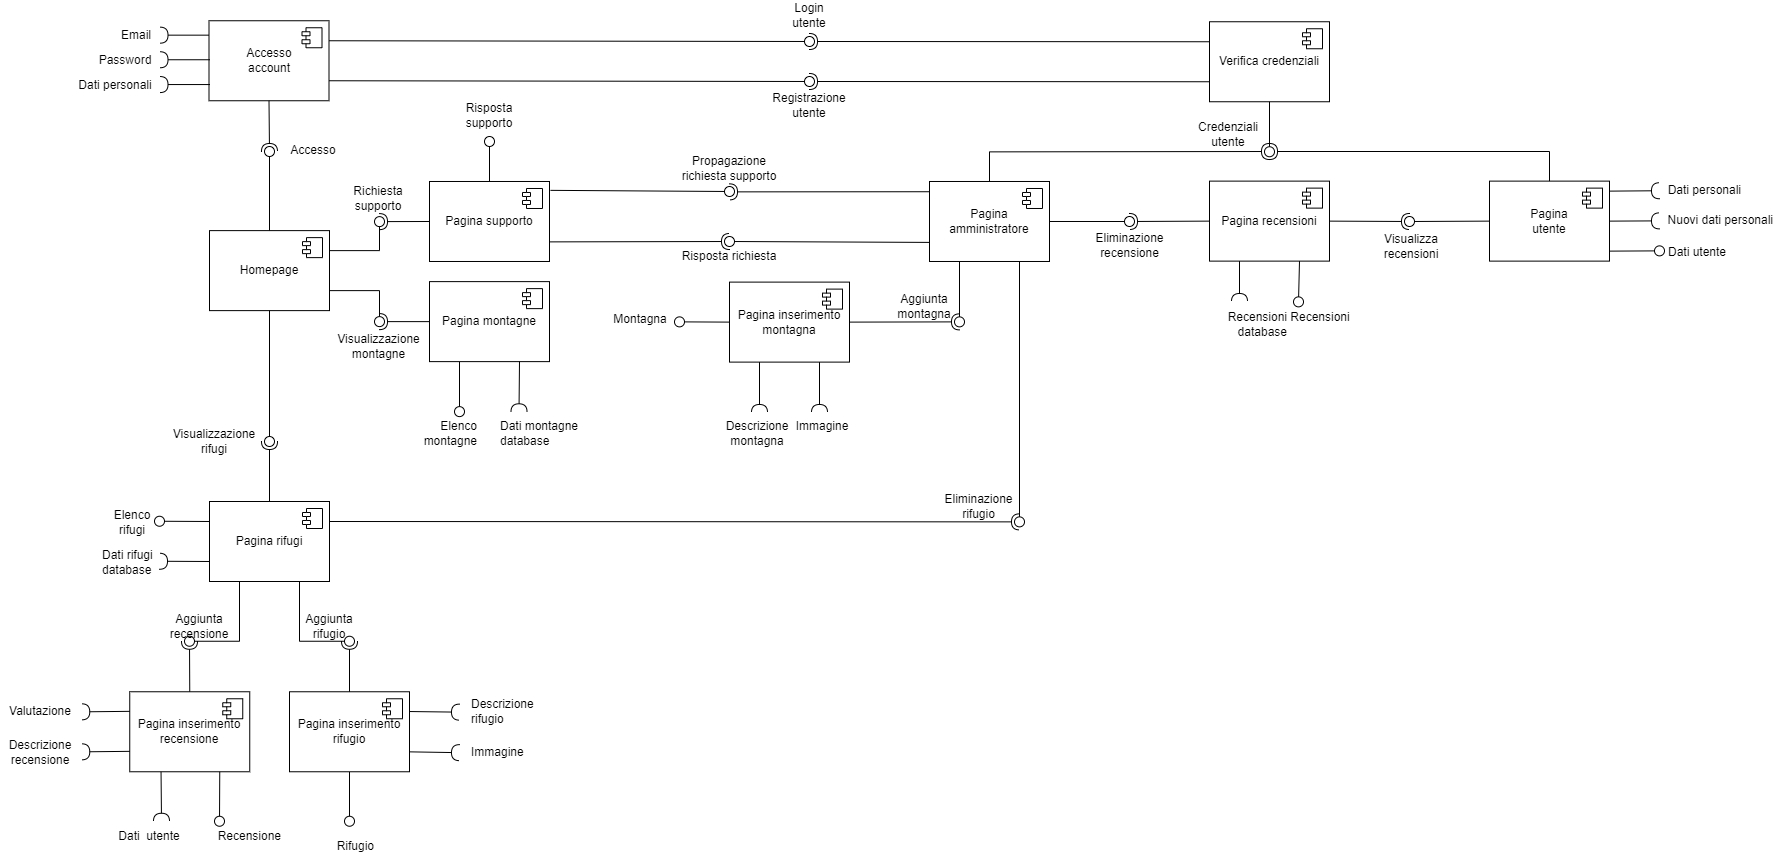
\includegraphics[width=1.4\textwidth, angle = 90]{
    img/diagramma_componenti.png}
    \caption{Diagramma componenti}
\end{figure}

\end{document}